\documentclass{article}
\usepackage[utf8]{inputenc}
\usepackage[margin=2cm]{geometry}
\usepackage{fontspec}
%\setmainfont{Noto Sans}

\usepackage{graphicx}
\usepackage{wrapfig}
\usepackage{float}
\usepackage{subcaption}

\usepackage{tikz}
\usetikzlibrary{positioning}

\title{Tesina PCTO}
\author{Gabriele Barola}
\date{A.S. 2021/2022}

\begin{document}
\maketitle
\tableofcontents

\section{Introduzione}
\subsection{Premessa}
Considerata la situazione di pandemia e le conseguenti restrizioni, l'attività
del PCTO è stata svolta senza una vera e propria alternanza presso un'azienda
esterna ma all'interno della scuola durante il mese di giugno del 2021.

L'attività è stata distribuita su due settimane durante le quali abbiamo avuto
la possibilità di approfondire alcune tecnologie a scelta, solitamente
non trattate nel corso.

L'attività proposta dal docente è stata lo sviluppo di semplici sistemi basati
su microcontrollori ESP8266 e ESP32 con il linguaggio di programmazione
\textbf{MicroPython} ed è proseguita durante l'anno scolastico con lo
sviluppo di un progetto.
\subsection{ESP32 e MicroPython}
ESP32 è una famiglia di microcontrollori prodotta da espressif, con l'enorme
vantaggio di avere a bordo un modulo per la connettività Wi-Fi e Bluetooth, che
la rende ottima per lo sviluppo di sistemi IoT.

Ne esitono diversi modelli con specifiche tecniche leggermente differenti e sono
inoltre disponibili svariate schede che mirano a renderne l'utilizzo,
soprattutto in fase di progettazione, il più semplice possibile, integrando
sistemi di alimentazione e programmazione tramite USB e rendendola compatibile
con la tecnologia THT.


\begin{figure}[H]%
    \centering
    \begin{subfigure}{0.49\textwidth}
        \centering
        \includegraphics[scale=0.4]{introduzione/esp32.png}%
        \caption{Scheda basata su ESP32}
    \end{subfigure}
    \begin{subfigure}{0.49\textwidth}
        \centering
        \caption{Caratteristiche tecniche di base}
        \begin{tabular}{|c|c|}
            \hline
            Internal clock frequency & 40MHz        \\
            \hline
            Ram                      & 520Kb        \\
            \hline
            Rom                      & 480Kb        \\
            \hline
            SPI Flash memory         & 4/8/16 Mb    \\
            \hline
            Supply voltage           & 3.0 to 3.6 V \\
            \hline
        \end{tabular}
    \end{subfigure}
    \caption{Esempio di ESP32}
\end{figure}

L'hardware più moderno e prestante rispetto ad altri microcontrollori rendono
ESP32 un'ottima scelta per quanto riguarda l'utilizzo di MicroPython, un
firmware particolare che una volta caricato sulla scheda ne permette la
programmazione tramite un linguaggio interpretato quasi totalmente compatibile
con l'implementazione x86 di Python.
\subsection{Descrizione del progetto}
Cercando di collegare l'attività del PCTO con le tematiche trattate in
educazione civica durante l'anno, ho deciso di sviluppare un sistema in grado di
monitorare i parametri necessari per mostrare all'utente in modo semplice lo
stato dell'impianto elettrico della propria abitazione e lo storico dei consumi,
con l'obiettivo di incentivare un un utilizzo più consapevole dell'energia
elettrica.

Il progetto unisce in unico pacchetto tutte le funzionalità di seguito riportate
e analazzite nello specifico successivamente:

\begin{itemize}
    \item Misurazione del valore efficace della tensione di rete;
    \item Misurazione della corrente circolante nell'impianto;
    \item Analisi della natura del carico;
    \item Misurazione della frequenza della tensione di rete;
    \item Visualizzazione dei dati in tempo reale su webserver;
    \item Visualizzazione dello storico dei consumi con grafici interattivi;
\end{itemize}

\section{Circuito di misurazione della corrente}
\subsection{Considerazioni}
L'impianto preso in esame è quello di unas tipica abitazione monofamiliare con
contratto da 3kW o 4.5kW. Considerando il caso limite possiamo calcolare la
corrente massima erogabile in condizioni standard: $4500/230 = 19.6A$.

Scegliendo \textbf{25A} come portata massima per la misura ci si assicura che il
dispositivo sia in grado di misurare i consumi in modo accurato anche in caso di
un temporaneo sovraccarico.

Con l'obiettivo di rendere l'installazione del dispositivo meno invasiva
possibile è stato utilizzato un trasduttore ad effetto Hall che ne permettesse
la messa in opera senza dover necessariamente essere posto in serie all'intero
impianto.
\subsection{Trasduttore di corrente CSLA2CD}

\begin{wrapfigure}[9]{l}{0.4\textwidth}
    \centering
    \includegraphics[scale=0.3]{corrente/csla2cd.png}
\end{wrapfigure}


Il trasduttore di corrente ad effetto Hall \textbf{CSLA2CD} è in grado di misurare la
corrente che lo attraversa senza la necessità di un collegamento fisico con
l'impianto. Il principio di funzionamento si basa sulla misura del campo
magnetico generato dal conduttore (in cui il trasduttore è immerso) piuttosto
che dell'intensità di corrente effettiva. Il passaggio di corrente all'interno
di un conduttore determina infatti la presenza di un campo magnetico avente
linee di campo concentriche e modulo proporzionale all'intensità di corrente.

\vspace{12mm}

Quando alimentato con una tensione di $8V_{DC}$ fornisce un'uscita in tensione sinusoidale con offset del tipo:

\begin{equation}
    V_o = 4 + 0.0327 \cdot I_{picco}
\end{equation}

L'alimentazione a 8V viene realizzata tramite uno stabilizzatore di tensione
LM7808 (come mostrato in figura \ref{fig:8v}) e l'uscita del trasduttore viene disaccoppiata
con un buffer prima di passare al circuito di condizionamento.

\begin{figure}[H]
    \centering
    \begin{subfigure}{0.49\textwidth}
        \centering
        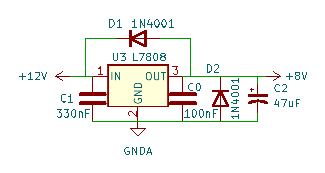
\includegraphics[scale=1.3]{corrente/lm7080.eps}
        \caption{Circuito di alimentazione 8V}
        \label{fig:8v}
    \end{subfigure}
    \begin{subfigure}{0.49\textwidth}
        \centering
        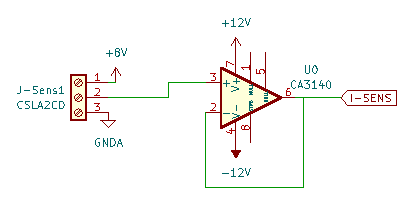
\includegraphics[scale=1.3]{corrente/buffer_csla2cd.eps}
        \caption{Buffer}
    \end{subfigure}
    \caption{Collegamento CSLA2CD}
\end{figure}
\subsection{Circuito di condizionamento}
\subsubsection{Obiettivo}
Per adattare il segnale del traduttore al circuito di misura e conversione
trattato nella sezione \ref{sec:adc} è necessario passare da una forma d'onda
come quella mostrata in figura \ref{fig:sign_trasd} ad un segnale sinusoidale
con $V_{eff(Max)} = 5V$ (fondoscala dell'adc) senza componente continua come
mostrato in figura \ref{fig:sign_adattato}.

\begin{figure}[H]
    \centering
    \begin{subfigure}{0.49\textwidth}
        \centering
        \includegraphics[scale=0.5]{corrente/sign_trasd.png}
        \caption{Uscita CSLA2CD}
        \label{fig:sign_trasd}
    \end{subfigure}
    \begin{subfigure}{0.49\textwidth}
        \centering
        \includegraphics[scale=0.5]{corrente/sign_adattato.png}
        \caption{Segnale condizionato}
        \label{fig:sign_adattato}
    \end{subfigure}
    \caption{Segnale di partenza e condizionato in condizioni di corrente massima}
\end{figure}

\subsubsection{Schema a blocchi}

\begin{figure}[H]
    \centering
    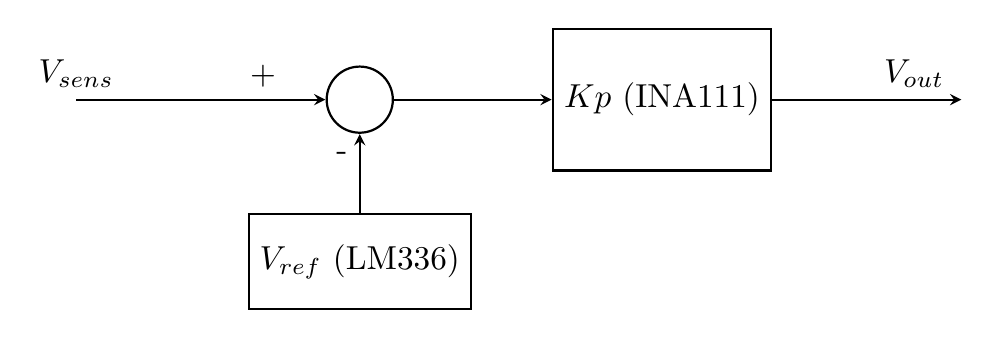
\begin{tikzpicture}[thick, scale=1.2, every node/.style={scale=1.2}]
        \node[
            draw,
            circle,
            minimum size=0.7cm
        ](sum) at (0,0){};

        \node[
            draw,
            below=1cm of sum,
            minimum width=1.5cm,
            minimum height=1cm
        ](ref){$V_{ref}$ (LM336)};

        \node[
            draw,
            right=2cm of sum,
            minimum width=2cm,
            minimum height=1.5cm
        ](gain){$Kp$ (INA111)};

        \draw [-stealth](-3,0) -- (sum.west)
        node[near end,above]{+}
        node[at start ,above]{$V_{sens}$};

        \draw [-stealth](ref.north)--(sum.south)
        node[near end, left]{-};

        \draw [-stealth](sum.east)--(gain.west);

        \draw [-stealth](gain.east) -- ++ (2,0)
        node[near end, above]{$V_{out}$};
    \end{tikzpicture}
\end{figure}

\subsubsection{Tensione di riferimento}
Per rimuovere l'offset di $V_{cc}/2 = 4V$ introdotto dal trasduttore, è stata
applicata all'ingresso invertente dell'amplificatore per strumentazione una tensione di
riferimento di pari valore generata da un LM336z2.5 opportunamente amplificato
secondo lo schema che segue.

\begin{figure}[H]
    \centering
    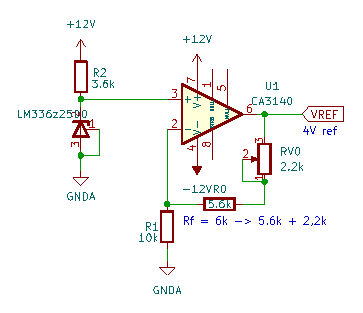
\includegraphics[scale=1.5]{corrente/ref.eps}
    \caption{Circuito di generazione tensione di riferimento}
\end{figure}

\subsubsection{Condizionamento con amplificatore per strumentazione}
Un amplificatore per strumentazione \textbf{INA111} è utilizzzato per rimuove la
tensione di offset e amplificare in modo adeguato il segnale per riportarlo al
caso in figura \ref{fig:sign_adattato}

\begin{figure}[H]
    \centering
    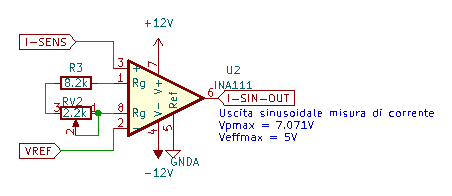
\includegraphics[scale=1.5]{corrente/ina.eps}
    \caption{Circuito di condizionamento}
\end{figure}


\subsection{Realizzazione}
Dopo aver tenuto conto di alcuni accorgimenti come l'inserimento di consensatori
per il disaccoppiamento e i terminali necessari per collegarsi agli altri
circuiti è stato disegnato un PCB non definitivo ma utile come riferimento per
la realizzazione del circuito su scheda millefori.

\begin{figure}[H]
    \centering
    \begin{subfigure}{0.49\textwidth}
        \centering
        \includegraphics[scale=0.25]{corrente/top.pdf}
        \caption{Stampa Copper Top}
    \end{subfigure}
    \begin{subfigure}{0.49\textwidth}
        \centering
        \includegraphics[scale=0.25]{corrente/bottom.pdf}
        \caption{stampa Copper Bottom}
    \end{subfigure}
    \caption{Stampe piste e serigrafia}
\end{figure}

%%AGGIUNGERE STAMPE 3D

\subsection{Taratura}

\end{document}